\title{Group 26 Report: Rotten Potatoes} % Title
\author{郑时飞 \\ 朱伯源 \\ 李易 \\ 汪明杰 \\ 施天昊}% Author
\date{\today}% Date

\documentclass[11pt]{article}
\usepackage[margin=1in]{geometry}
\usepackage{vmargin}
\usepackage{url}
\usepackage{datetime}
\usepackage[utf8]{inputenc}
\usepackage{CJKutf8}
\usepackage{graphicx}
\usepackage{mathtools}
\usepackage{float}
\usepackage[colorlinks,linkcolor=blue,urlcolor=blue]{hyperref}


\makeatletter 
    \newcommand\fcaption{\def\@captype{table}\caption}
\makeatother
\setmarginsrb{3 cm}{2.5 cm}{3 cm}{2.5 cm}{1 cm}{1.5 cm}{1 cm}{1.5 cm}

\makeatletter
\let\thetitle\@title
\let\theauthor\@author
\let\thedate\@date
\makeatother

\usepackage{graphicx, bm}
\graphicspath{{graphics/}}
\usepackage{geometry}
\geometry{left=5cm,top=5cm,right=0cm,bottom=0cm}

\usepackage[colorlinks,linkcolor=blue]{hyperref}

\begin{document}
\begin{CJK*}{UTF8}{gbsn}

\begin{titlepage}
    \centering
    \vspace*{0.5 cm}
    
\includegraphics[scale = 0.75,width=6cm]{CUHK}\\[1.0 cm]
    \textsc{\large The Chinese University of Hong Kong, Shenzhen}\\[1.5 cm] 
    \textsc{\Large CSC 3170}\\[0.5 cm] 
    \textsc{\large Database System}\\[0.5 cm]
    \rule{\linewidth}{0.2 mm} \\[0.4 cm]
    { \huge \bfseries \thetitle}\\
    \rule{\linewidth}{0.2 mm} \\[0.6 cm]
    
    \begin{minipage}{0.4\textwidth}
        \begin{flushleft} \large
            \emph{Authors:}\\
            郑时飞 \\ 朱伯源 \\ 李易 \\ 施天昊 \\ 汪明杰
            \end{flushleft}
    \end{minipage}~
    \begin{minipage}{0.4\textwidth}
            \begin{flushright} \large
            \emph{Student Number:} \\
            119010465 \\ 119010485 \\ 119010156 \\ 120090472 \\ 119010300
        \end{flushright}
    \end{minipage}\\[2 cm]
    {\large \thedate}\\[2 cm]
 
    \vfill
    
\end{titlepage}

\tableofcontents
\pagebreak

\rmfamily
\section{Introduction}
\paragraph{}As an art and commercial work, movies have become pursuits of many people and generated tremendous value. Currently, there are two types of online movie platforms. On the one hand, platforms including Rotten Tomatoes and Douban gives people rich information regarding movies. On the other hand, sites like Netflix offers precise, personalized recommendation to users. Such a recommendation strategy allows users to discover more films they enjoy and attracts more users to the platform.
\paragraph{}However, currently, no site combines the strengths of the mentioned movie sites. Besides, existing popular movie websites are full of quarrels and controversies from the perspective of the community environment. The movie recommendation sare influenced deeply by the advertising, not the quality of films. Therefore, to satisfy the real requirements of movie lovers, we build a movie database called \textbf{Rotten Potatoes}, based on which, users can talk about their reviews on the movie freely. It also offers plenty of searching functions and personalized recommendations from the platform. 
\paragraph{}We use python packages \textbf{\textit{Requests}}, \textbf{\textit{BeautifulSoup}} to obtain the required data from IMDB, store it in a MySQL database. Then we build our searching functions and personalized moive recommendations on those data. We also build a user-friendly web using \textbf{\textit{amis}} as the frontend and \textbf{\textit{express}} as the backend.
\section{Design}
In this section, we focus on the design of Entity-Relationship Model, 
the reduction from ER diagram into relational schemas, constraint and index.

\subsection{Entity-Relationship Model}
As shown in the \hyperref[ERD]{ER digram}, there are 6 entities and 5 relationships. 
\paragraph{Entity ``movies''}
To store id, name, cover url, introduction, release year and genres of a movie, where genres is a multivariate attribute. Identified by id. 
\paragraph{Entity ``directors''}
To store id, name, photo url, introduction and birth date of a director. This entity has a one-to-many relationship ``direct'' with the entity ``movies'', which means a director can directs multiple movies and a movie can be directed by only one director in our assumption. Identified by id. 
\paragraph{Entity ``actors''}
To store id, name, photo url, introduction and birth date of an actor. This entity has a many-to-many relationship with the entity ``movies'', which means an actor can act in multiple movies and a movie can be acted by multiple actors in our assumption. Identified by id. 
\paragraph{Entity ``users''}
To store id, name, avatar url, password of a user. This entity has a many-to-many relationship with the entity ``movies'', which means a user can comment on multiple movies and a movie can be commented by multiple users in our assumption. Identified by id. 
\paragraph{Entity ``characters''}
To store movie id (of the movie where this character appears), actor id (of the actor who acts as this character), id, character name of a character. This entity is a weak entity identified by entity ``movies'' through relationship ``appear'' and entity ``actors'' through relationship ``act as'', and also by its own id, which means a character can be acted by exactly one actor and appear in exactly one movie in our assumption (we treat characters of the same name appearing in multiple movies or acted by multiple actors as multiple different characters for simplicity). Note that since this entity is also identified by its own id, it is allowed that an actor acts as multiple characters in the same movie. 
\paragraph{Entity ``comments''}
To store movie id (of the movie commented by this comment), user id (of the user who makes this comment), id, rate (from 0 to 10), content and comment date of a comment. This entity is a weak entity identified by entity ``movies'' and entity ``users'', and also by its own id, which means a comment is on exactly one movie and is made by exactly one user in our assumption. Note that since this entity is also identified by its own id, it is allowed that a user makes multiple comments on the same movie. 

\begin{figure}[h]
\centering
\label{ERD}
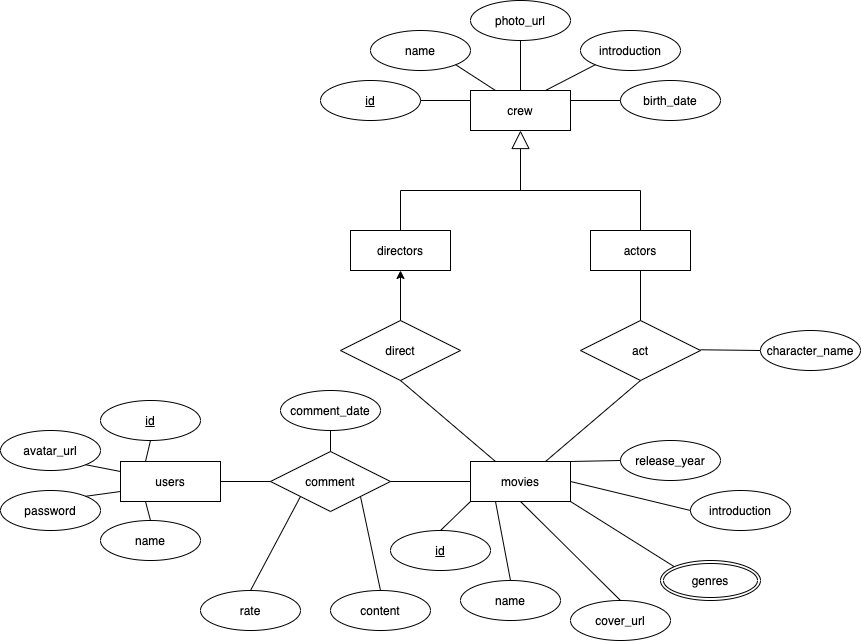
\includegraphics[width=0.8\textwidth]{er.png}
\caption{ER Diagram}
\end{figure}

\subsection{Relational Schema}
As shown in the \hyperref[RelationalSchema]{relational schema digram}, there are 7 schemas. 

The following reductions are made:
\begin{itemize}
\item The attribute ``genres'' in entity ``movies'' is reduced to schema ``genres'' with attributes ``genres\_name'' and ``movie\_id'' as a foreign key, both of which forms a primary key to make sure no redundant genres of a movie.
\item The relationship ``direct'' between entity ``movies'' and ``directors'' is reduced to attribute ``director\_id''as a foreign key in schema ``movies'' so that a movie is directed by exactly one director. 
\item All attributes identifying the entity are reduced to primary keys.
\item ``movie\_id'', ``actor\_id'' of entity ``characters'', ``movie\_id'', ``user\_id'' of entity ``comments'' are reduced to foreign keys in their schemas referencing their corresponding identifying strong entities. 
\end{itemize}

\begin{figure}[h]
\centering
\label{RelationalSchema}
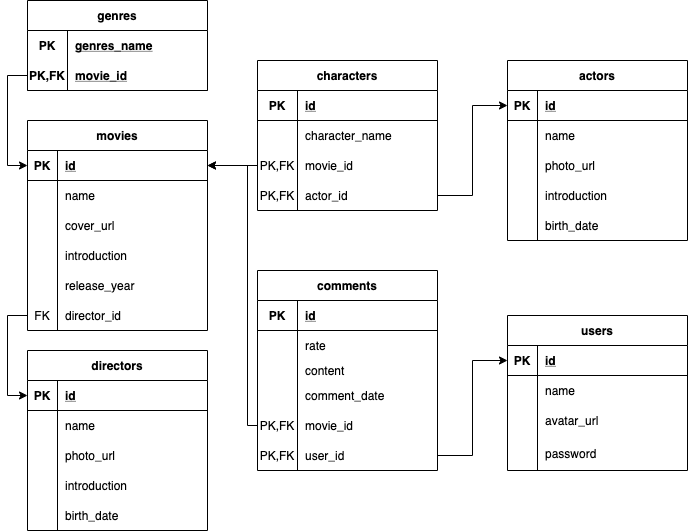
\includegraphics[width=0.8\textwidth]{schema.png}
\caption{Relational Schema Diagram}
\end{figure}

\subsection{Constraint}
3 types of constraints are further added:
\paragraph{Not Null Constraints}
\begin{itemize}
\item All ``id'' attributes as they are primary key and thus automatically becoming not null.
\item ``name'' attribute of schema ``movies''.
\item ``name'' and ``director\_id'' attributes of schema ``directors'', as a movie is directed by exactly one director.
\item ``name'' attribute of schema ``actors''.
\item ``name'' and ``password'' attributes of schema ``users''.
\item ``actor\_id'', ``movie\_id'' and ``character\_name'' attributes of schema ``characters'', as it is a weak entity of schemas ``actors'' and ``movies''.
\item ``user\_id'', ``movie\_id'', ``rate'', ``content'' and ``comment\_date'' attributes of schema ``comments'', as it is a weak entity of schemas ``users'' and ``movies''.
\item ``genres\_name'', ``movie\_id'' attributes of schema ``genres'', as it is a multivariate attribute of schema ``movies''.
\end{itemize}
\paragraph{Unique Constraint}
A unique constraint is added to ``name'' attribute of schema ``users'' as by our assumption there should be no repeating user names. 
\paragraph{Check Constraint}
A check constraint is added to ``rate'' attribute of schema ``comments'' to make sure the rate is from 0 to 10.

\subsection{Index}
The following attributes are indexed to make search faster:
\begin{itemize}
\item ``name'' and ``release\_year'' attributes of schema ``movies''.
\item ``name'' and ``birth\_date'' attributes of schema ``directors''.
\item ``name'' and ``birth\_date'' attributes of schema ``actors''.
\item ``name'' attribute of schema ``users''.
\end{itemize}

\section{Implementation}
\subsection{Frontend}
The frontend of our project is constructed using \textbf{\textit{amis}}, a low-code front end framework. It can generate a website using json configurations, which is suitable for developing a light-weight and agile application like this project.\par
When users access the webpage, they will be directed to the Login page, where registered user can input user name and password to log in. We also added support for new user registration.
After login, users can see the  main structure of our website, which features a navigation pannel on the left side and the content on the right. We constructed the following pages:
\begin{itemize}
    \item Movie: a list of all the movies with their name and posters. Each movie is a "Card" widget linking to the movie detail page.
    \item Actor: a list of all the actor/actresses, also implemented using the "Card" widget, containing links to the detailed information.
    \item Director: a list of all the directors implemented similarly as the \textbf{Actor} page
    \item Comment: this page contains the latest comments that users release.
    \item Me: a portal for users to edit their information. Including updating avatar, name, password. This page also contains a list of movies recommended to the user.
    \item Search: to search for movies/actors/user, we implemented three different pages. The details will be discussed in \textbf{Sample Queries} section.
\end{itemize}
\par \hyperref[moviePage]{Fig.3} shows the movie page of our website. Since our application is user-oriented, the UI of our website is very concise and user-friendly.\par

\begin{figure}[h]
    \label{moviePage}
    \centering
    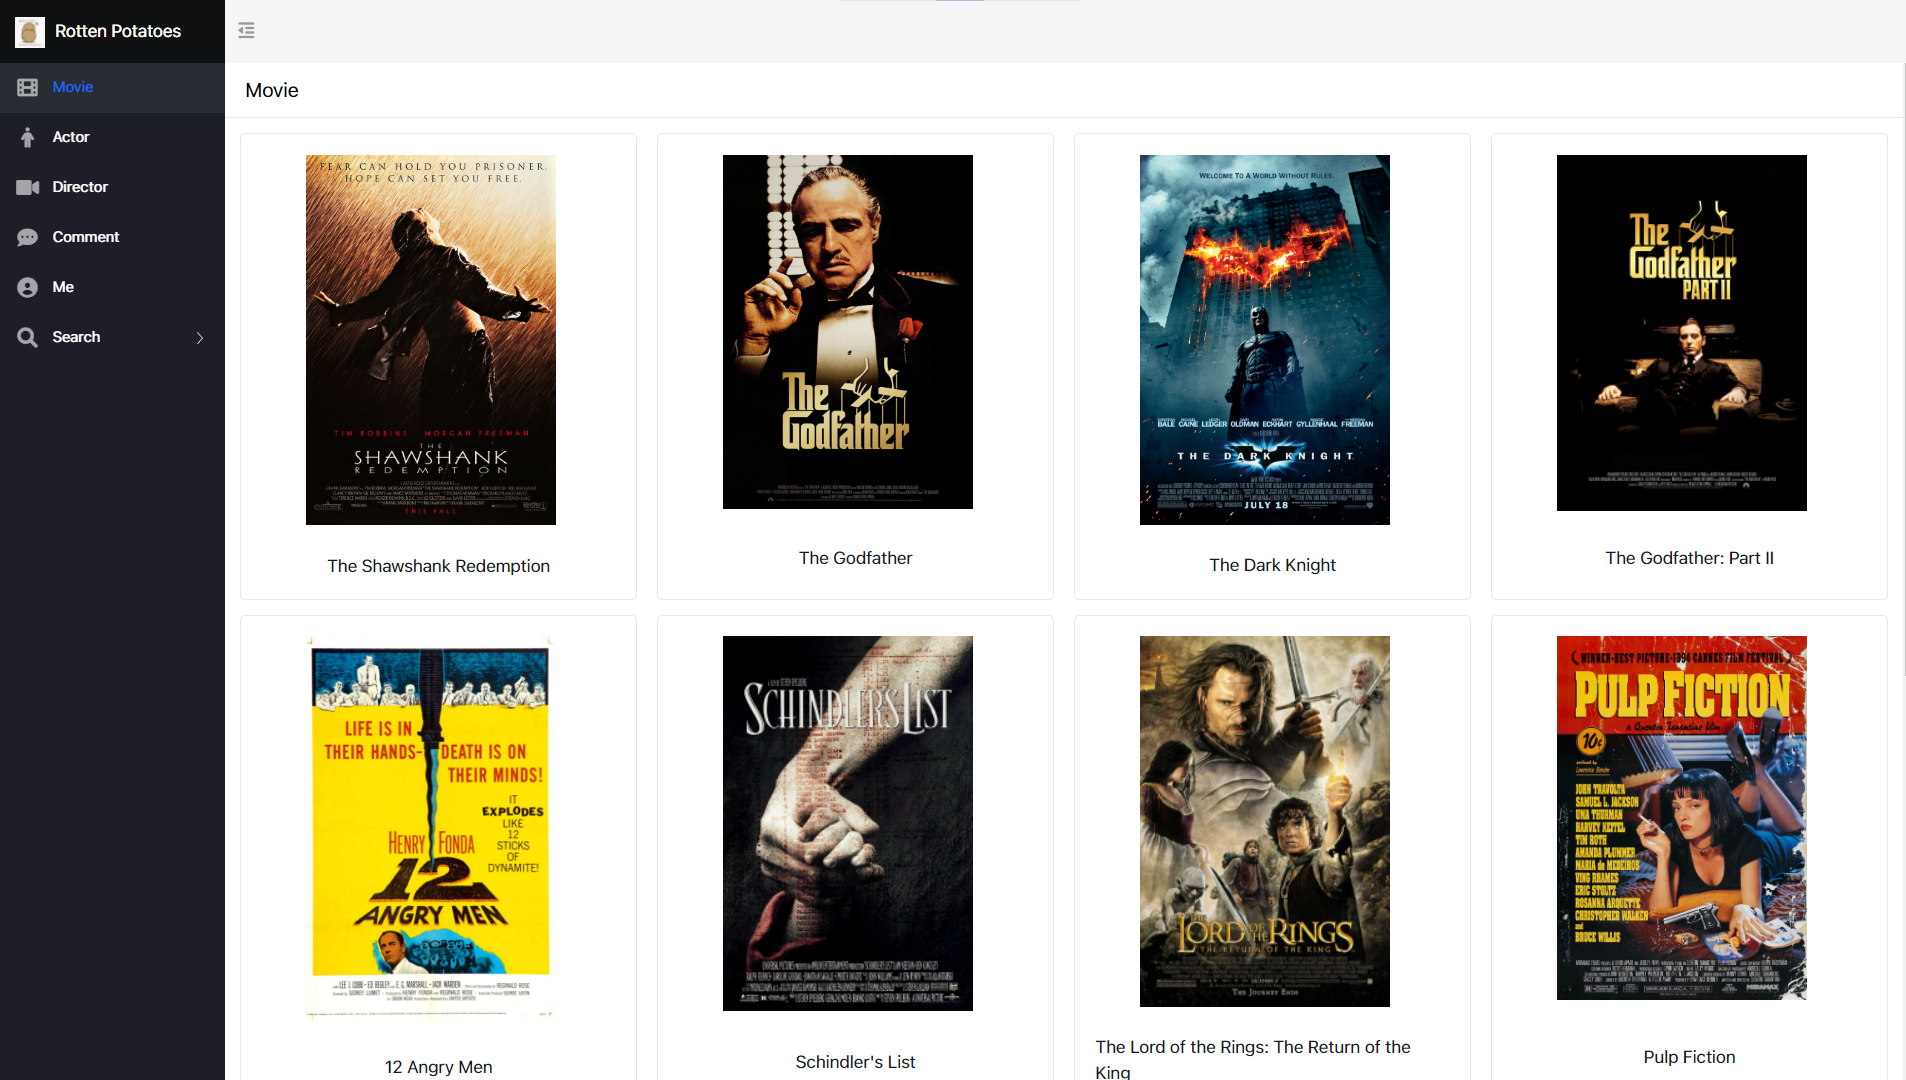
\includegraphics[width=0.8\textwidth]{website.png}
    \caption{Movie page of the website}
\end{figure}

\subsection{Backend}
%Backend of this project is implemented through the \textbf{\textit{express}} package of nodejs. During the initialization, the `init.js' will read data from CSV files and create queries to batch-insert records into corresponding tables.
\paragraph{Connect to MySQL in Nodejs}
The query functions in our database are written in javascript language. They can be found in the corresponding files in the \textbf{services} folder. To maximize reusability, we wrote a template query function in \textbf{query.js} using the \textit{mysql} module of Node.JS. The template function will first access the \textbf{.env} file for database configuration(e.g., the port on which MySQL server is running, the logging username and password). Then, instead of establishing and closing connections to the database on every execution, the template creates a connection pool. Requests from the frontend will pass the query as rest parameter to the template function, which will then issue the query and return the results (and errors, if any) back to the frontend.
\begin{figure}[h]
    \label{moviePage}
    \centering
    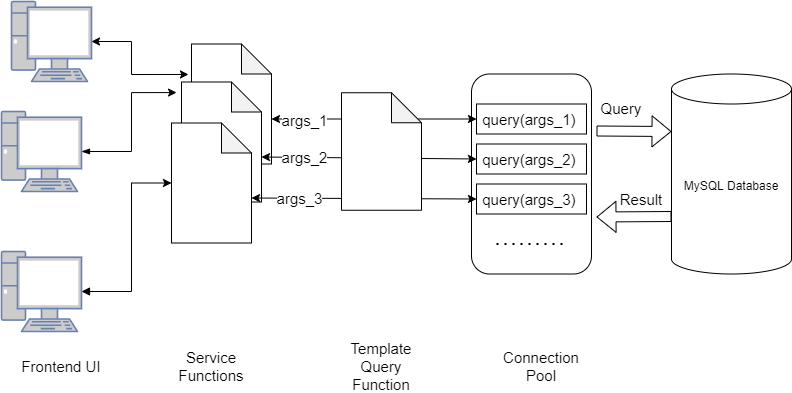
\includegraphics[width=0.8\textwidth]{sqlconnect.png}
    \caption{Database connection flowchart}
\end{figure}
\paragraph{Provide API by Express Router}
We use the \textbf{express} library to provide APIs for frontend users. All the routers are written in the \textbf{router/index.js}. Whenever users access certain page, it will match a router in the file, which triggers the corresponding handler function. For example, after log in, the user will see the \textit{Movie} page, which contains a list of movies in the database. When user click on any of the movie poser , the frontend will request for page \underline{./movie/detail/<movie_id>}, matching a router in index.js (line 26). The router then calls the corresponding handler function, in this case, the \textit{getMovieDetail()} function in \textbf{movie.js}, which directs the user to the corresponding movie detail page.
\paragraph{Access Control by jsonwebtoken}
auth/auth.js调用jsonwebtoken包sign和verify token,\\
services/auth.js中login路由函数调用signToken生成token给前端,\\
auth中间件函数调用verifyToken验证前端传来的token是否正确/过期(不是很重要,看不懂留着我写)

\subsection{Web Crawler}
\subsubsection{Basic Workflow}
To populate our database with real-world data, we wrote a web crawler to scrap information from IMDB's Top 250 Movie Chart. The crawler is written in Python. It uses the requests library to send https requests. The desired fields are acquired through parsing the page using Beautiful Soup 4 library.
The detailed process is as follows (see \hyperref[crawler]{Fig.4}):\par

\begin{enumerate}
    \item Access the Top 250 Chart, where all the URLs to the detailed movie pages are located
    \item Traverse through the chart. For every movie of the chart:
    \begin{enumerate}
        \item Access the detailed movie page, where information regarding the movie can be found.
        \item From the detailed movie page, we access the casting information.\\ For the director:
        \begin{itemize}
            \item For directors yet to be recorded, access the detailed director page, where information regarding the director can be found.
        \end{itemize}
        For the actors/actresses who casted in this movie:
        \begin{itemize}
            \item Access the detailed actor/actress page and find detailed information.
        \end{itemize}
        \item The comment section locates at the bottom of the movie page. We collect the rating, comments from this section.
        \item For each comment, we acquire the user information by accessing their homepage.
    \end{enumerate}
\end{enumerate}

\begin{figure}[h]
    \label{crawler}
    \centering
    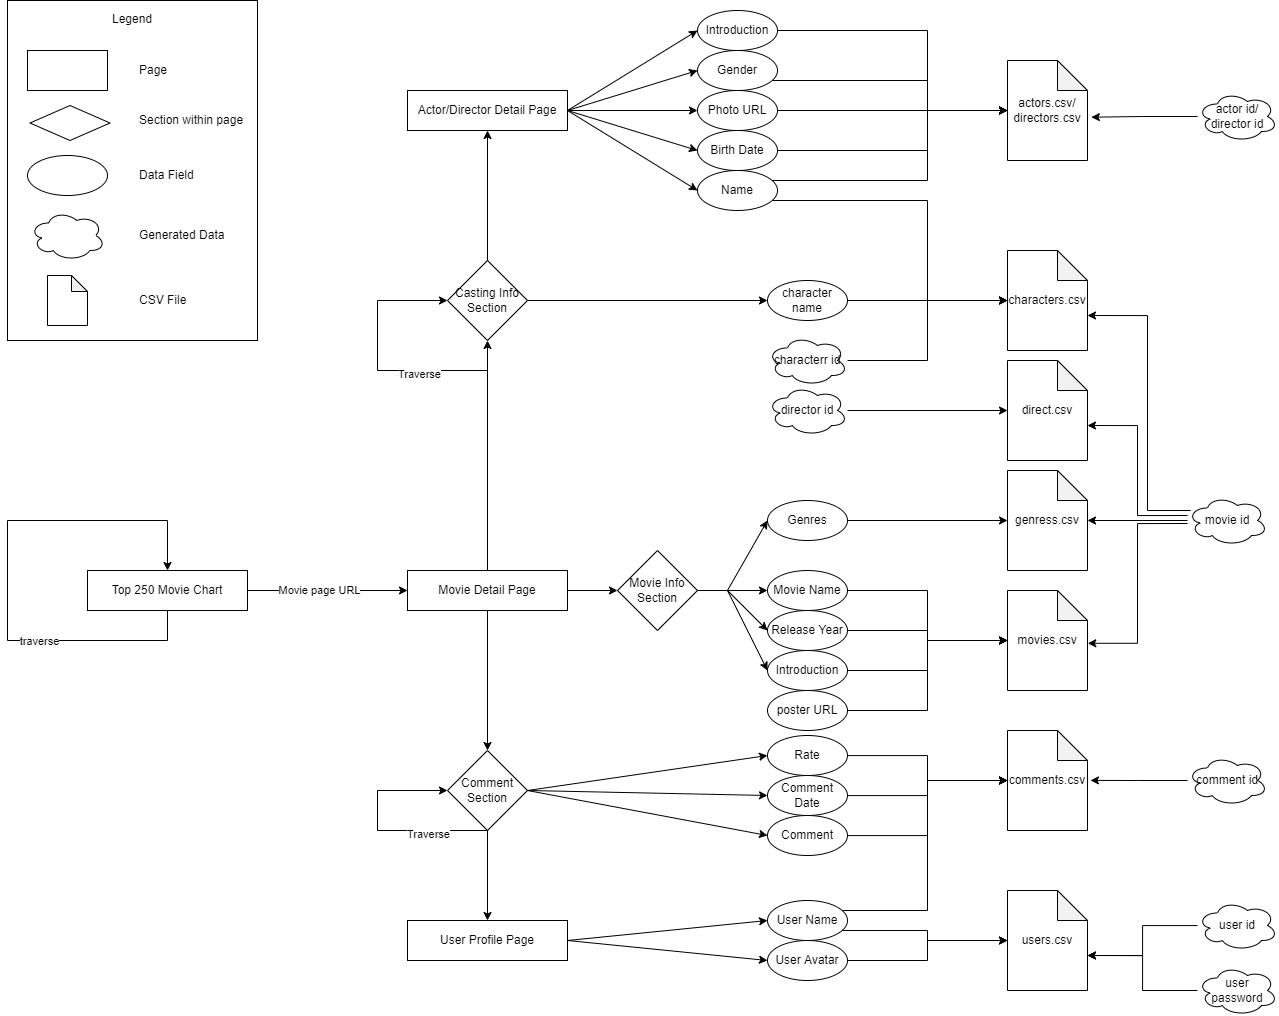
\includegraphics[width=0.8\textwidth]{crawler_flowchart.png}
    \caption{Web crawler flowchart}
\end{figure}

\subsubsection{Encountered Problems and Solutions}
During the scrapping process, we encountered some issues.
\begin{itemize}
    \item The same director or actor/actress can participate in different movies. Therefore, we keep a mapping relationship and check wheter we have record the same person's information. This step is done through hashing the person's name, which takes O(1) complexity.
    \item We do not have access to each user's password, so we randomly generate a password for each user we scrapped from IMDB. The password is a random combination 5 to 10 numbers and characters.
    \item Some actors' birth date cannot be achieved from their detailed page. We leave them as NULL.
    \item The gender of the movie stars is not explicitely listed on their detail page. However, by seeking their role in the movie (i.e, actor/actress), we can acquire their gender.
\end{itemize}
\subsection{Sample Queries}
李易写下这里(每个功能大概怎么实现的)
\subsubsection{User related}
\subsubsection{CRUD on movies, actors and directors}
\subsubsection{Comments related}
\subsection{Data Analysis}
\subsubsection{Recommendation System with Restricted Boltzmann Machines}

In 2007, Hinton showed that Restricted Boltzmann Machines (RBMs) can be successfully applied to Netflix dataset and do personalized movie recommendations (Hinton et al., 2007). This paper was given in a DDA course project, but that project requires only the basic RBM without biases, conditional RBM, neighborhood. We reproduce the model proposed by Hinton (see \hyperref[RBM]{Fig.5}) in this project to do recommendation. We use Contrastive Divergence (CD) to approximate the maximum likelihood of the parameters by Gibbs sampling.
\begin{itemize}
    \item First get the visible movies ratings $ \bm{V} $ of the user.
    \item Sample the hidden units to binary numbers by probability given by \\ $ p(h_j = 1 | \bm{V}, \bm{r}) = \sigma(c_j + \sum_{i = 1}^m \sum_{k = 1}^K v_i^k W_{ij}^k + \sum_{i = 1}^M r_i D_{ij}) $, where $ \sigma(x) = \frac{1}{1 + e^{-x}}  $.
    \item Reconstruct the visible units by $ p(v_i^k = 1 | \bm{h}) = softmax(b_i^k + \sum_{j = 1}^F h_j W_{ij}^k) $, \\where $ softmax(x_k) = \frac{e^{x_k}}{\sum_{l= 1}^K e^{x_l}} $. Notice that we only reconstruct the movies the use has rated.
    \item Update the parameters by the origin data and reconstructed data. For example, $ \Delta W_{ij}^k = \epsilon (<v_i^k h_j>_{data} - <v_i^k h_j>_T) $, where $ T $ represents the number of runs we do Gibbs sampling.
    \item Prediction is much the same as doing Gibbs sampling except that we can reconstruct (predict) missing ratings.
\end{itemize}
\begin{figure}[htbp]
\centering
\label{RBM}
\begin{minipage}[t]{0.45\textwidth}
\centering
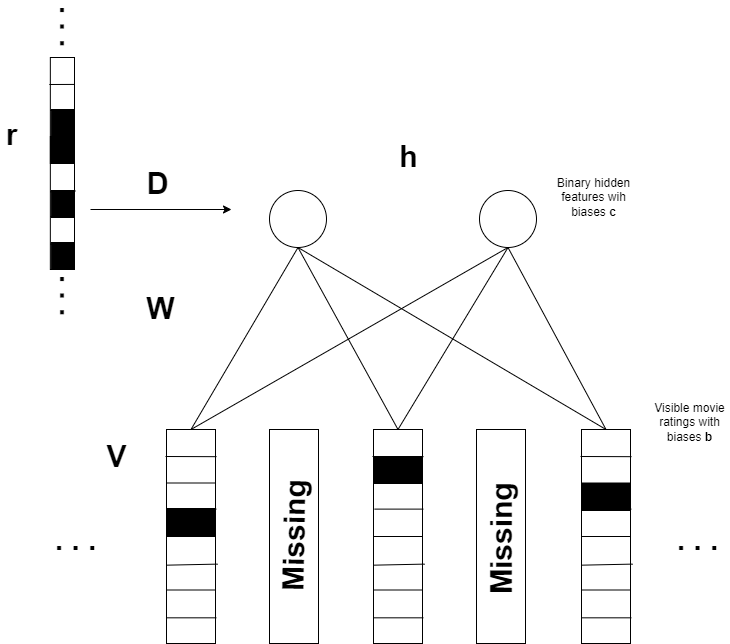
\includegraphics[width=6cm]{conditionalRBM.png}
\caption{Conditional RBM}
\end{minipage}
\begin{minipage}[t]{0.45\textwidth}
\centering
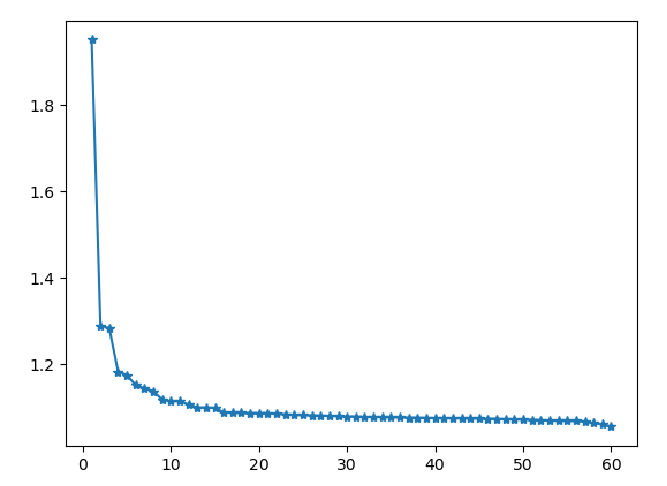
\includegraphics[width=6cm]{RBMResult.png}
\caption{Train RMSE vs. Epochs}
\end{minipage}
\end{figure}
\hyperref[RBM]{Fig.6} shows the evolution of Root Mean Squared Error during training. We achieve a RMSE of 1.04. Every time the user enters \textbf{Me} page on our website, the system will automatically predict the ratings over all movies and recommend the top 8 movies to the user in \textbf{Guess you like} module. See \hyperref[recommend]{Fig.7} for an example.
\begin{figure}[h]
    \centering
    \label{recommend}
    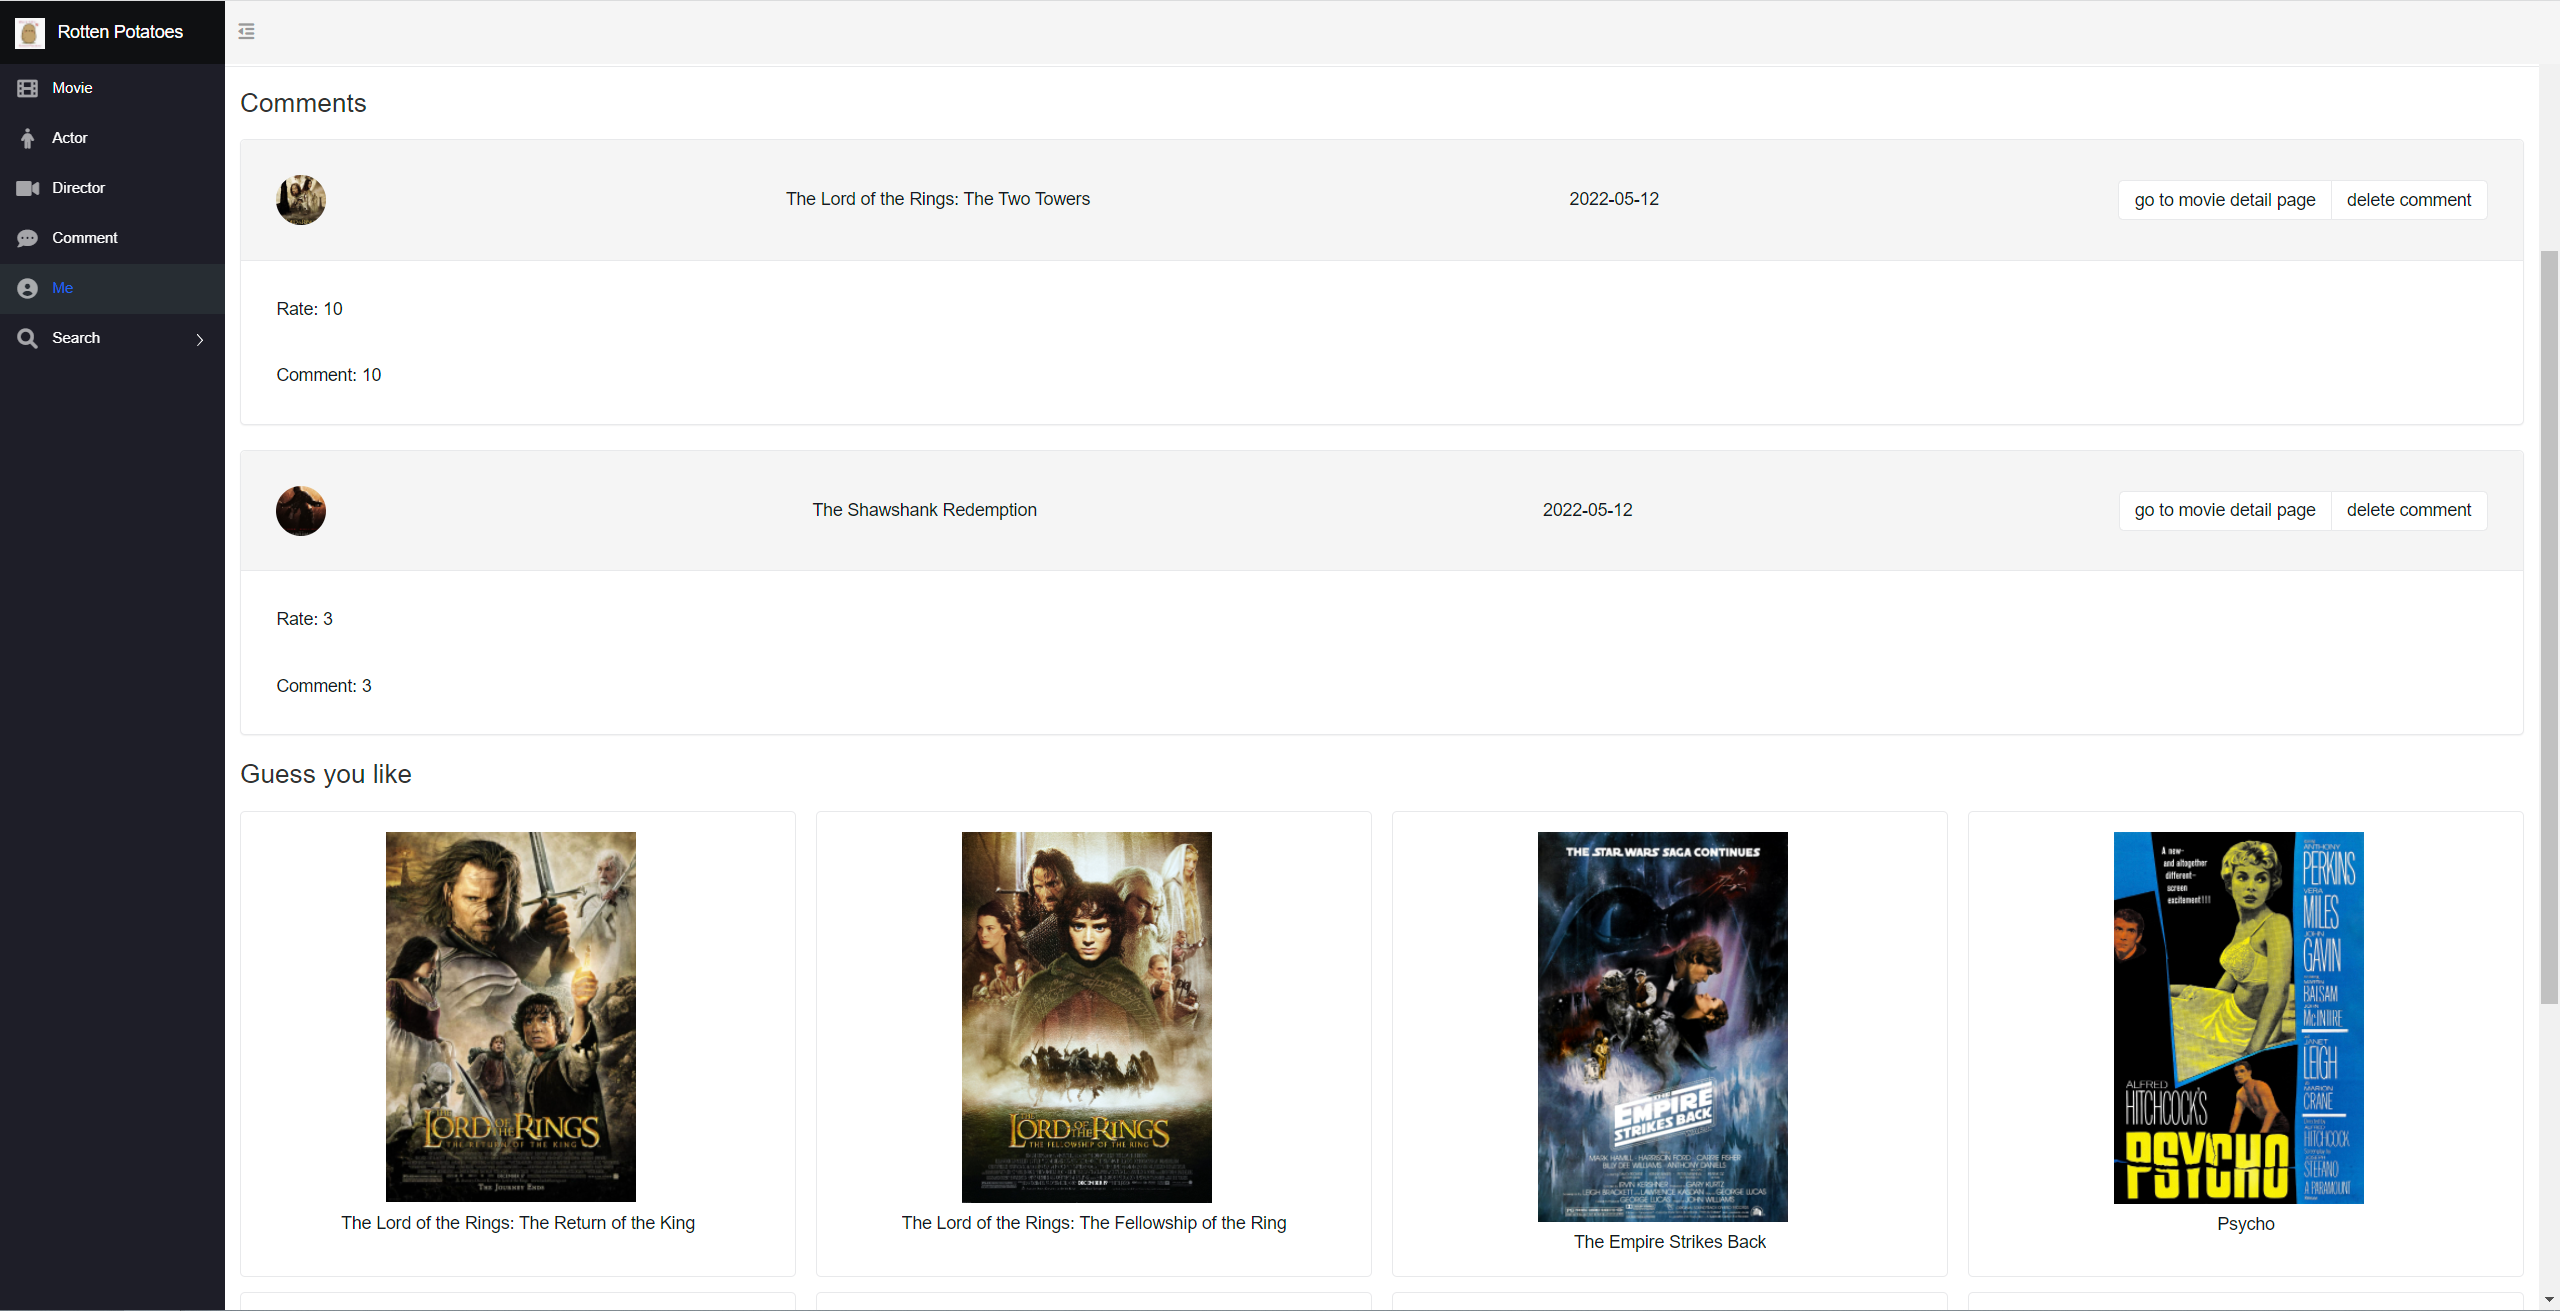
\includegraphics[width = 0.7\textwidth]{recommendation.png}
    \caption{Personalized Movie Recommendation}
\end{figure}
\subsubsection{Neighbourhood Model}
Users have their preferences and tend to give similar ratings to movies of the same kind. In other words, movies are correlated and we can utilize this property to improve our predictions $ \hat{R} $ :
\begin{itemize}
    \item Define an error matrix by $ \widetilde{R} = R - \hat{R} $
    \item Define similarity between two movies by their column features (user ratings): $ d_{A B}=\frac{\tilde{r}_{A}^{T} \widetilde{r}_{B}}{\left\|\widetilde{r}_{A}\right\|_{2}\left\|\widetilde{r}_{B}\right\|_{2}} $
    \item Predict the error of one movie through the errors of its neighbours: $ \hat{\tilde{r}}_{i A}=\frac{1}{\sum_{B \in S}\left|d_{A B}\right|} \sum_{B \in S} d_{A B} \widetilde{r}_{i B}  $, where $ S $ is the set of neighbours (with high absolute similarities) of $ A $.
    \item Improve our RBM predictions by $ R_{u m}^{*}=\hat{R}_{u m}+\hat{\tilde{r}}_{u m} $ for each $ (user, movie) $ pair desired.
\end{itemize}
We improve the RMSE from 1.04 to 1.02. The improvement is not high because our matrix is sparse. In our data set, many users only give one rating, so it is hard to construct a well defined similarity matrix. The other reason is that we crawl high-rating movies and the biases are not large to give a performance boost. However, we are still able to leverage the data and get some insight into the movie ratings. 

For the movie \textit{The Godfather}, movie \textit{The Godfather: Part II} has a high similarity (based on the difference between real rating and predicted rating) of $ 0.9999 $, which is expected. However, movie \textit{The Lord of the Rings: The Return of the King} has a similarity of $ -0.9999 $ while the movie \textit{The Lord of the Rings: The Fellowship of the Ring} has a similarity of $ 0.9999 $. This is counter intuitive and we should look into the data. We have three users giving ratings to both \textit{The Godfather} and \textit{The Lord of the Rings: The Return of the King}. The ratings are $ (10, 10) $, $ (10, 10) $ and $ (8, 10) $, respectively. For \textit{The Godfather} and \textit{The Lord of the Rings: The Fellowship of the Ring}, the rating pairs are all $ (10, 10) $. 8 is a relatively low rating in our dataset, hence the algorithm concludes that they are high negatively correlated.

\section{Result}
李易写下这里(贴网页截图介绍下功能就ok了)

\section{Conclusion}
\paragraph{} In this project we build a movie database based on a large amount of data collected from \textbf{IMDB}. Additional attention is paid to assure a \textbf{BCNF} form is kept for every entity in our database, thus the redundancy part is eliminated. We also \textbf{implement useful functions} for our users to search for moives, casts or other users using name,  time information, rate(only movies) and genres(only movies) as the keyword.
\paragraph{} In order to improve user experience and replace the complex database operations by a few simple mouse clicks from users, we build a user friendly website. Based on that, abundant \textbf{personalized interaction behaviors} can be achieved, which serves our users more conveniently. We hold an integral process of account management for users. Users can add comments to a movie and rate on it as well as discover their appreciated reviews or users.
\paragraph{} It is common for a movie database to recommend movies that the users have potential interest in. However,  how to make a personalized recommendation lists of high quality is always a problem. We use a lot of techniques in the data analysis to satisfy the needs from users . We build a \textbf{Restricted Boltzmann Machines}  with \textbf{Neighbourhood model} and get gratifying results.
\section{Self Evaluation}
In this part, we evaluate the advantages and disadvantages of our project/
\subsection{What we have achieved}
\begin{enumerate}
\item Build a database conforming to the low redundancy paradigm
\item Implement and optimize many necessary  searching functions
\item Create a user-friendly website to lower the bar of use
\item Feed the database with a suitable amount of data and design a proper data analysis algorithm to satisfy personalized requirements
\end{enumerate}
\subsection{Future Improvements}
\begin{enumerate}
\item More information about movies, directors, actors can be added to the database. For example, for actors we may add their nationality and Oscar nominations; for movies we may add its budget and the classification (PG13, NC17).
\item More interaction functions can be add, like ``like'' a movie or ``subsrcibe'' a user. We can also add functions like ``want to watch'' a movie or ``watched'' a movie without commenting on it. This information can be utilized in conditional RBM to provide better recommendation (Hinton et al, 2007). Currently, we have the algorithm implemented but the information is unknown. 
\item In the future, we plan to distinguish the users of our platform. We will allow a common user to upgrade as administrator, which will reduce the effort to maintain and supervise the comments other users post.
\item Currently the web crawler is implemented using synced requests, which reduced its performance. In the future, we will write the crawler using async requests to speed up the crawling performance and acquire more data for our database.
\end{enumerate}

\section{Contribution}
Each of us contributed 20\% to the whole project.

\end{CJK*}
\end{document}
